\clearpage
\section{Quantum efficiency editor}
The quantum efficiency editor simulates both EQE and IQE.  The configuration window can be used to set the voltage at which EQE and IQE are performed.
\begin{figure}[H]
\centering
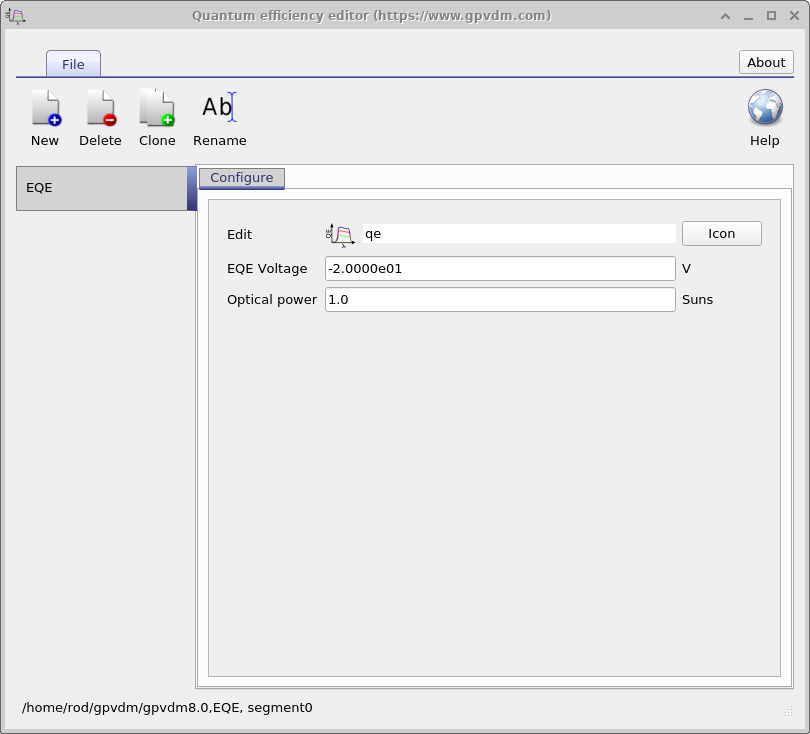
\includegraphics[width=0.7\textwidth,height=0.5\textwidth]{./images/sim_editors/qe_editor.png}
\caption{The quantum efficiency editor window}
\label{fig:qeeditor}
\end{figure}

\subsection{Outputs}

\begin{table}[H]
\begin{center}
\begin{tabular}{ |c|c| } 
 \hline
	File name 		& 	Description  \\ 
 \hline
	eqe.csv 		&	Wavelength v.s. EQE \\ 
	E\_eqe.csv		&	Photon energy v.s. EQE \\ 
	E\_eqe\_norm.csv	&	Photon energy v.s. Normalized EQE  \\ 
	iqe.csv			&	Wavelength v.s. IQE \\ 
	E\_iqe.csv		&	Photon energy v.s. IQE \\ 
	lam\_Gn.csv		&	Wavelength v.s. Average charge carrier generation rate \\ 
 \hline
\end{tabular}
\caption{Files produced by the Suns-Jsc simulation}
\label{tab:suns_jsc_output}
\end{center}
\end{table}
